\documentclass[border=14pt]{standalone}
\usepackage[T1]{fontenc}
\usepackage[scaled=1.0]{helvet}
\renewcommand{\familydefault}{\sfdefault}
\usepackage{amsmath}
\usepackage{sansmath}
\sansmath
\hyphenpenalty=10000
\exhyphenpenalty=10000
\usepackage{xcolor}
\usepackage{tikz}
\usetikzlibrary{arrows.meta,positioning,calc,fit,backgrounds}
\definecolor{cblue}{HTML}{CFE2F8}
\definecolor{cpeach}{HTML}{F9DDD2}
\definecolor{cmint}{HTML}{D3EFE1}
\definecolor{cgrey}{HTML}{ECEBE7}
\definecolor{cline}{HTML}{6B6B6B}
\definecolor{clabel}{HTML}{555555}
\tikzset{
  blk/.style={draw=cline, line width=1.1pt, rounded corners=6pt, align=center, inner sep=6pt, minimum height=2.1cm, text width=#1},
  blk/.default=5.0cm,
  data/.style={blk=#1, fill=cgrey}, data/.default=5.0cm,
  ctrl/.style={blk=#1, fill=cblue}, ctrl/.default=5.0cm,
  path/.style={blk=#1, fill=cpeach}, path/.default=5.0cm,
  ana/.style={blk=#1, fill=cmint}, ana/.default=5.0cm,
  wire/.style={-{Stealth[length=9pt,width=7pt]}, draw=cline, line width=1.1pt},
  dwire/.style={wire, dashed},
  lab/.style={font=\normalsize, text=clabel},
  lane/.style={font=\large\bfseries, text=clabel},
}
\newcommand{\nt}[2]{{\LARGE #1}\\[3pt]{\Large #2}}

\begin{document}
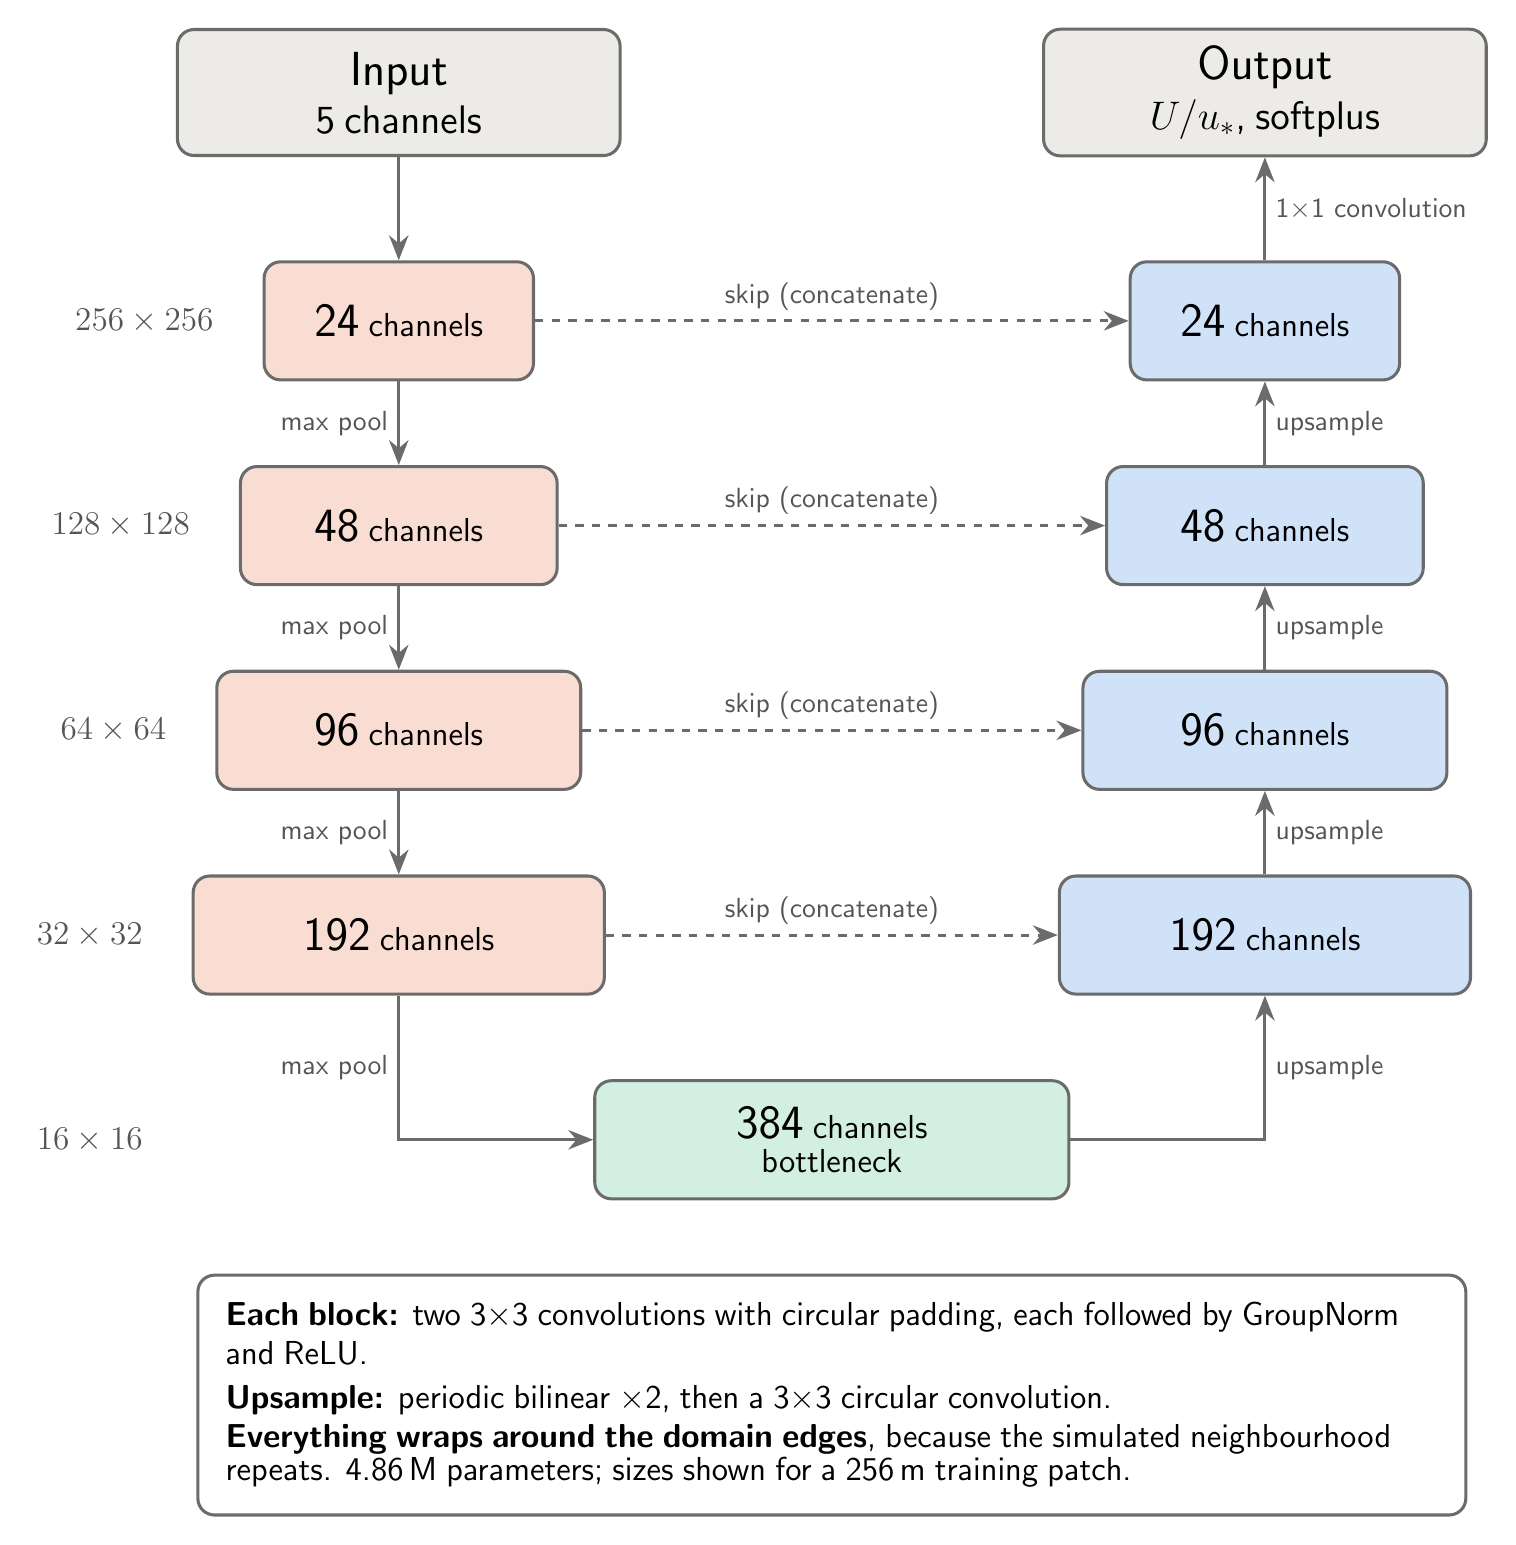
\begin{tikzpicture}
\def\ex{0}\def\dx{11.0}\def\dy{2.6}
\foreach \i/\c/\w/\s in {0/24/3.0/256, 1/48/3.6/128, 2/96/4.2/64, 3/192/4.8/32} {
  \node[path=\w cm, minimum height=1.5cm] (e\i) at (\ex,-\i*\dy) {{\LARGE \c} {\large channels}};
  \node[ctrl=\w cm, minimum height=1.5cm] (d\i) at (\dx,-\i*\dy) {{\LARGE \c} {\large channels}};
  \node[lab, anchor=east] at ($(e\i.west)+(-0.5,0)$) {\large $\s \times \s$};
  \draw[dwire, draw=cline] (e\i.east) -- node[lab, above] {skip (concatenate)} (d\i.west);
}
\node[ana=5.6cm, minimum height=1.5cm] (b) at (\dx/2,-4*\dy) {{\LARGE 384} {\large channels} \\ {\large bottleneck}};
\node[lab, anchor=east] at ($(e3.west)+(-0.5,-\dy)$) {\large $16 \times 16$};
\foreach \i/\j in {0/1,1/2,2/3} {
  \draw[wire] (e\i) -- node[lab, left] {max pool} (e\j);
  \draw[wire] (d\j) -- node[lab, right] {upsample} (d\i);
}
\draw[wire] (e3.south) |- node[lab, pos=0.25, left] {max pool} (b.west);
\draw[wire] (b.east) -| node[lab, pos=0.75, right] {upsample} (d3.south);
\node[data=5.2cm, minimum height=1.6cm] (in) at (\ex,2.9) {\nt{Input}{5 channels}};
\node[data=5.2cm, minimum height=1.6cm] (out) at (\dx,2.9) {\nt{Output}{$U/u_*$, softplus}};
\draw[wire] (in) -- (e0);
\draw[wire] (d0) -- node[lab, right] {1$\times$1 convolution} (out);
\node[draw=cline, line width=1.1pt, rounded corners=6pt, fill=white, align=left, text width=15.4cm, inner sep=10pt, anchor=north] at (\dx/2,-4*\dy-1.7) {\large
\textbf{Each block:} two 3$\times$3 convolutions with circular padding, each followed by GroupNorm and ReLU.\\[2pt]
\textbf{Upsample:} periodic bilinear $\times$2, then a 3$\times$3 circular convolution.\\[2pt]
\textbf{Everything wraps around the domain edges}, because the simulated neighbourhood repeats. 4.86\,M parameters; sizes shown for a 256\,m training patch.};
\end{tikzpicture}
\end{document}
